%========================================================================
% Modelo para elaboracao de textos academicos: TCC, dissertacoes e teses
% Elaborado pelo GISIS - Grupo de Imageamento Sismico e Inversao Sismica.
%========================================================================
\chapter{Resultados}
\label{ch:resultados}

\section{Inversão com malha esparsa}




\section{Inversão com malha refinada}






%Nessa seção, os resultados devem ser descritos de maneira objetiva, obedecendo uma sequência lógica, usando texto, figuras e tabelas. Ela deve ser organizada de tal forma que sejam destacadas as evidências necessárias para responder cada questão de pesquisa ou hipótese levantada. Deve ser escrita de forma concisa e objetiva.
%
%\begin{table}[h]
%    \vspace{0.2cm}
%    \centering
%    \caption{Tabela de parâmetros e valores.}
%    \begin{tabular}{c|c|c|c} 
%                    & Teste 1 & Teste 2 & Teste 3 \\ \hline
%        Parâmetro 1 & Valor 1 & Valor 2 & Valor 3 \\
%        Parâmetro 2 & Valor 4 & Valor 5 & Valor 6 \\
%        Parâmetro 3 & Valor 7 & Valor 8 & Valor 9 \\
%        Parâmetro 4 & Valor 10 & Valor 11 & Valor 12
%    \end{tabular}
%    %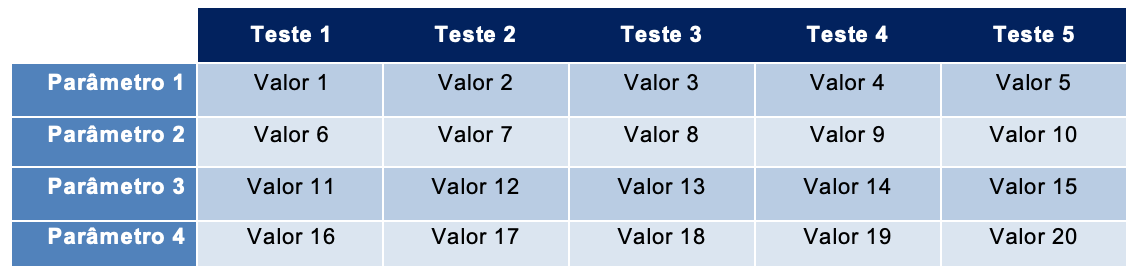
\includegraphics[width= \textwidth]{Imgs/Resultados/tabelaParametros.png} %também é possível inserir uma imagem de uma tabela (isso substitui o que esta no tabular)
%    \label{tabelaResultados}
%    \vspace{0.2cm}
%\end{table}
%
%Dicas:
%    \begin{itemize}
%        \item Quando uma hipótese ou questão de pesquisa é estabelecida, os dados do estudo são observados, coletados e analisados de forma que responda as questões. Caso uma abordagem mais simples esteja sendo utilizadas, essa análise é feita, visualizando figuras e tabelas, fazendo cálculos de média, desvio padrão, etc. Ao utilizar uma análise mais rebuscada, pode-se interpretar uma variedade de testes estatísticos com diferentes técnicas.
%        \item Escreva os resultados para mostrar o maior número possível de informações para o leitor em relação àqueles aspectos analisados e aos seus possíveis relacionamentos.
%    \item Organize os resultados com base na sequência de figuras e tabelas. Olhe para a tabela e figura e identifique três palavras-chave, isso vai auxiliar na escrita sobre aquela tabela ou figura.
%    \item A seção de resultados é feita com base no texto criado para descrever as informações relevantes identificadas, referenciando as figuras e tabelas sempre que possível. Deve-se conduzir o leitor de forma que fiquem claros os resultados do seu estudo, que vão depender do tipo de questão de pesquisa. Eles podem incluir tendências, diferenças, similaridades, correlações, mínimos, máximos, etc.
%    
%    \item Caso não encontre o resultado que esperava, isto pode ser algum erro na definição da hipótese, que precisa ser reformulada ou talvez tenha tropeçado em algo inesperado que precisa ser melhor investigado. Em qualquer um desses casos, os resultados são importantes mesmo que eles não dêem suporte a sua hipótese. Não considere que resultados diferentes do que se esperava são resultados ruins. Estudos elaborados com qualidade mesmo que gerem resultados “ruins” podem proporcionar importantes descobertas na área. Desta forma, escreva seus resultados honestamente!!!
%
%    \end{itemize}